\documentclass[a4paper,12pt]{article}
\usepackage[utf8]{inputenc}
\usepackage[ngerman]{babel}
\usepackage{textcomp}
\usepackage{listings}
\usepackage{graphicx}
\usepackage{tabularx}
\usepackage{pgfplots}
\usepackage{pgfplotstable} %Für Erstellung von Tabellen aus .csv-Datei
\usepackage[hidelinks]{hyperref}
\usepackage{gensymb}
\usepackage[figure]{hypcap} 
\usepackage[default,osfigures,scale=0.95]{opensans} %% Alternatively
%% use the option 'defaultsans' instead of 'default' to replace the
%% sans serif font only.
\usepackage[T1]{fontenc}
\usepackage{pdfpages}




\usepackage[left=2cm,right=2cm,top=2cm,bottom=2cm,includeheadfoot]{geometry}
\usepackage{fancyhdr}
\pagestyle{fancy}
\fancyhf{}


%Die Dokumentbasisdaten
\newcommand{\fak}{Fakultät für Technik}
\newcommand{\studGang}{Studiengang Technische Informatik}
\newcommand{\titel}{Endbericht Praxissemester}
\newcommand{\subtitel}{<Untertitel>}
\newcommand{\dokArt}{<Mein Abschlussbericht>} %Legt die Art des Dokumentes fest (Projektarbeit, Doktorarbeit, Laborbericht, etc)
\newcommand{\autor}{<Vorname Nachname>} %Name des Autors
\newcommand{\matnr}{<Matrikelnummer>} %Matrikelnummer
\newcommand{\abgabe}{<Abgabedatum>} %Abgabedatum
\newcommand{\Professor}{<Profesorname>} %Betreuender Professor
\newcommand{\Betreuer}{} %Weitere Betreuer




%Kopfzeile mittig
\fancyhead[L]{\leftmark}
%Linie oben
\renewcommand{\headrulewidth}{0.5pt}

%Fußzeile links bzw. innen
\fancyfoot[L]{\autor \  (Matr-Nr.: \matnr)}
%Fußzeile rechts bzw. außen
\fancyfoot[R]{\thepage}
%Linie unten
\renewcommand{\footrulewidth}{0.5pt}







\usepackage{tikz}
\usetikzlibrary{shapes.geometric, arrows}



%Deklaration
\tikzstyle{startstop} = [rectangle, rounded corners, minimum width=3cm, minimum height=1cm, text centered, draw=black, fill=red!10]
\tikzstyle{io} = [trapezium, trapezium left angle=70, trapezium right angle=110, minimum width=3cm, minimum height=1cm, text centered, draw=black, fill=blue!10]
\tikzstyle{process} = [rectangle, minimum width=3cm, minimum height=1cm, text centered, draw=black, fill=orange!10]
\tikzstyle{decision} = [diamond, minimum width=3cm, minimum height=1cm,  text centered, draw=black, fill=green!10]
\tikzstyle{arrow} = [thick,->,>=stealth]

%opening
\title{\titel}
\author{\autor (Matr-Nr.: \matnr)}
\date{01.09.2016}



\begin{document}

%\includepdf{img/deckblatt-hs.pdf} %Eventuell PDF vorher einfügen

%Diese Datei kann nicht allein kompiliert werden und dient nur zu Includezwecken.

%Verwendete Variablen 
% Bitte Folgenden Block kopieren und anpassen!
%Die Dokumentbasisdaten
%\newcommand{\fak}{Fakultät für Technik}
%\newcommand{\studGang}{Studiengang Elektrotechnik/Informationstechnik}
%\newcommand{\titel}{Der Dokumententitel}
%\newcommand{\subtitel}{Der Untertitel}
%\newcommand{\dokArt}{Laborbericht} %Legt die Art des Dokumentes fest (Projektarbeit, Doktorarbeit, Laborbericht, etc)
%\newcommand{\autor}{Sebastian Strittmatter} %Name des Autors
%\newcommand{\matnr}{311577} %Matrikelnummer
%\newcommand{\abgabe}{16.04.2015} %Abgabedatum
%\newcommand{\Professor}{Prof. Dr. rer. nat. Stefan Bernhard} %Betreuender Professor
%\newcommand{\Betreuer}{M.Sc. Andrej Sycev und Dipl.-Ing. Dieter Gann} %Weitere Betreuer

%---------------- BEGIN DECKBLATT ---------------------------------
\ifdefined\NoTitle

\else
\begin{titlepage}
\fi
\vspace*{-3.0cm}
%\begin{figure}[ht]
%  \centering
  
%  \caption{}
%\end{figure}

\begin{center}

\includegraphics[width=1.0\textwidth]{logo-hs.png}
 \Large \textbf{\fak}\\[1.5cm]
 
 \large \textbf{\studGang} \\[3.5cm]
 
 \LARGE \textbf{\titel} \\[0.5cm]
 \large \textit{\subtitel} \\[2.5cm]
 
 \textbf{\dokArt} \\[2.5cm]
 
\begin{tabular}{ll}
  \textbf{Professor} &  \Professor\\
  \textbf{Betreuer} & \Betreuer\\[1.5cm]
  \textbf{vorgelegt von} & \autor\\
 \textbf{Matrikelnummer} & \matnr\\[1cm]
 \textbf{Abgabetermin} & \abgabe
\end{tabular} \\[1.5cm]



                          
 
\end{center}


\ifdefined\NoTitle

\else
\end{titlepage}
\fi
%------------------ ENDE DECKBLATT ----------------------------------------------
\ifdefined\ShowTOC

\else
\renewcommand{\contentsname}{Inhalt}
\tableofcontents %Macht das Inhaltsverzeichnis
\fi

\pagebreak

\section{Einleitung}
\label{kap:Einleitung}
Das ist die Einleitung der Arbeit.
Der Text der Einleitung kommt einfach in \textbf{diese} die einleitung.tex


\section {Kapitel 1}
\label{kap:Kapitel 1}
Ein Text der Unter der Hauptüberschrift steht.

\subsection{Gliederungsebene 2}
\label{kap:Gliederungsebene 2}
Auch unter dieser Gliederungsebene gibt es einen kleinen Demotext.

%So fügt man ein Bild ein
\begin{figure}[h]
        \centering
        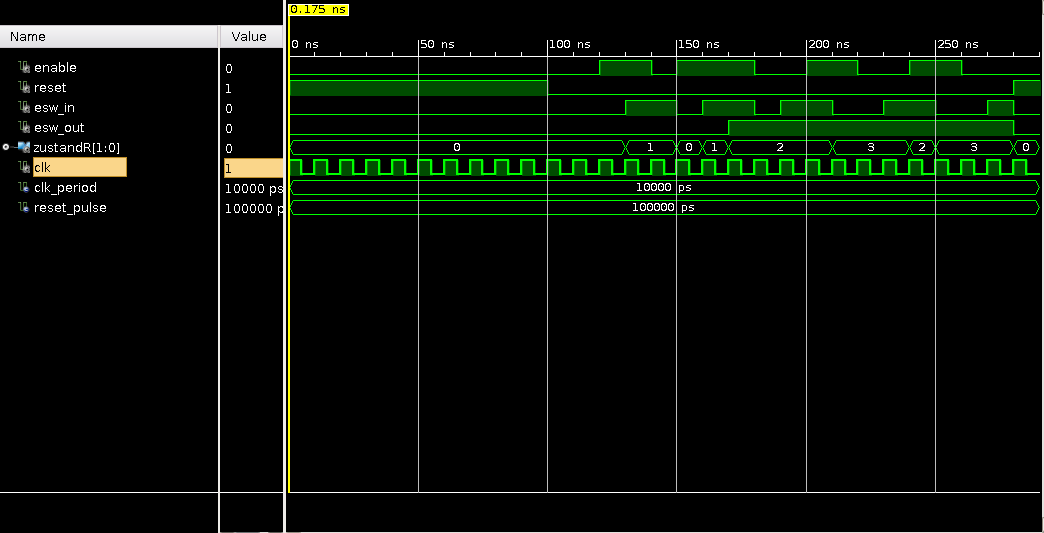
\includegraphics[scale=0.3]{img/simulation.png}
        \caption{Unterschiedliche Layouts aus der gleichen Logik}
        \label{fig:Different_Images}
\end{figure}




%Hier können weitere Kapitel hinzugefüht werden.


%% Verzeichnisse 
\cleardoublepage %Fügt eine leere Seite ein 
% \phantomsection
\addcontentsline{toc}{section}{\listfigurename} %Fügt Eintrag Abbildungsverzeichnis in Inhaltsverzeichnis ein
\listoffigures	%Abbildungsverzeichnis


\end{document}
